\documentclass[10pt]{article}
\usepackage[T1]{fontenc}
\usepackage{tgtermes}
\usepackage{graphicx}
\usepackage{natbib}
\usepackage{tocloft}
\usepackage[nottoc]{tocbibind}
\usepackage{siunitx}
\usepackage{listings}
\usepackage[breaklinks]{hyperref}
\usepackage{tocloft}
\usepackage[font=small,skip=7pt]{caption}
\usepackage{xcolor}

\definecolor{codegreen}{rgb}{0,0.6,0}
\definecolor{codegray}{rgb}{0.5,0.5,0.5}
\definecolor{codepurple}{rgb}{0.58,0,0.82}
\definecolor{backcolour}{rgb}{0.95,0.95,0.92}

\lstdefinestyle{mystyle}{
    backgroundcolor=\color{backcolour},
    commentstyle=\color{codegreen},
    keywordstyle=\color{magenta},
    numberstyle=\tiny\color{codegray},
    stringstyle=\color{codepurple},
    basicstyle=\ttfamily\footnotesize,
    breakatwhitespace=false,
    breaklines=true,
    captionpos=b,
    keepspaces=true,
    numbers=left,
    numbersep=5pt,
    showspaces=false,
    showstringspaces=false,
    showtabs=false,
    tabsize=2
}

\lstset{style=mystyle}

\renewcommand{\lstlistlistingname}{List of \lstlistingname s}
\renewcommand{\bibsection}{\section*{Bibliography}}
\renewcommand{\contentsname}{Table of Contents}
\renewcommand\cftsecafterpnum{\vskip10pt}
\renewcommand{\bibsection}{\section{\bibname}}
\renewcommand{\cftsecleader}{\cftdotfill{\cftdotsep}}

\PassOptionsToPackage{hyphens}{url}
\urlstyle{same}
\def\Urlmuskip{0mu}
\def\UrlBreaks{\do\/\do-}
\hypersetup{
  colorlinks = true,
  urlcolor = blue,
  linkcolor = black,
  citecolor = black,
  breaklinks=true,
  pdfpagemode=UseOutlines,
  bookmarksopen=true,
  bookmarksopenlevel=2,
  bookmarksnumbered=true
  }

  \title{\textbf{WebAssembly and the \linebreak  Wizards of Hogwarts}}
  \author{Daniel Burger}
  \date{7. November 2020}

\begin{document}
\pagenumbering{roman}
\counterwithin{lstlisting}{section}
\counterwithin{figure}{section}
\counterwithin{table}{section}

\maketitle
\thispagestyle{empty}
\begin{sloppypar} % For better line breaks

  \pagebreak
  \begin{abstract}
    There is a new kind in the web development hood: WebAssembly. It is fast, portable, supported by the big players and should allow making the world wide web the biggest software platform in existence. It doesn’t matter if you are an experienced software architect or a front-end developer — everyone will be able to profit from WebAssembly’s existence.

    In this article, we will look at what WebAssembly is, how it works and how it works alongside its sibling JavaScript.

  \end{abstract}
  \thispagestyle{empty}
  \pagebreak

  \pagenumbering{Roman}
  \tableofcontents
  \pagebreak

  \listoffigures
  \pagebreak
  \listoftables
  \pagebreak
  \addcontentsline{toc}{section}{\lstlistlistingname}
  \lstlistoflistings
  \pagebreak

  \pagenumbering{arabic}
  \section{Introduction}
  \label{sec:introduction}

  \begin{figure}[ht]
    \centering
    
\includegraphics[width=\textwidth]{figures/001.jpg}
    \caption{Harry Potter dress form with a black jacket \citep{unsplash_beautiful_2018}}
    \label{fig:cover}
  \end{figure}

  On the 17th of June 2015, Brendan Eich — the inventor of JavaScript — and the teams behind Mozilla, Chromium, Edge and WebKit presented a new browser standard: WebAssembly, a portable and highly efficient byte-code compilation target for high-level languages such as C++ and Rust \citep{eich_asmjs_2015}.

  However, what does this mean? What is the reason that WebAssembly should exist in the first place? Should JavaScript developers be worried now? And what do the wizards of Hogwarts have to do with it?

  \section{Web Development Back Then}
  \label{sec:back-then}

  Back in the day when you could call yourself web developer because you only understood HTML, web development itself was a rather interactionless and static field of business. Netscape Communications, one of the establishing companies who built the world wide web as we know it today, soon realised that websites lacked to be interactive and dynamic \citep{cassel_brendan_2018}. They wanted the web to be a new form of a distributed operating system rather than just a simple HTML document-accessing application on your computer.

  Marc Andreessen, who was the founder of Netscape Communications, proposed that HTML needed some kind of “scripting language” that was approachable — something you could glue directly into the markup. A language that is easy to use by newbie programmers who didn’t want to handle compiler errors or strictly-typed syntax.

  \begin{figure}[ht]
    \centering
    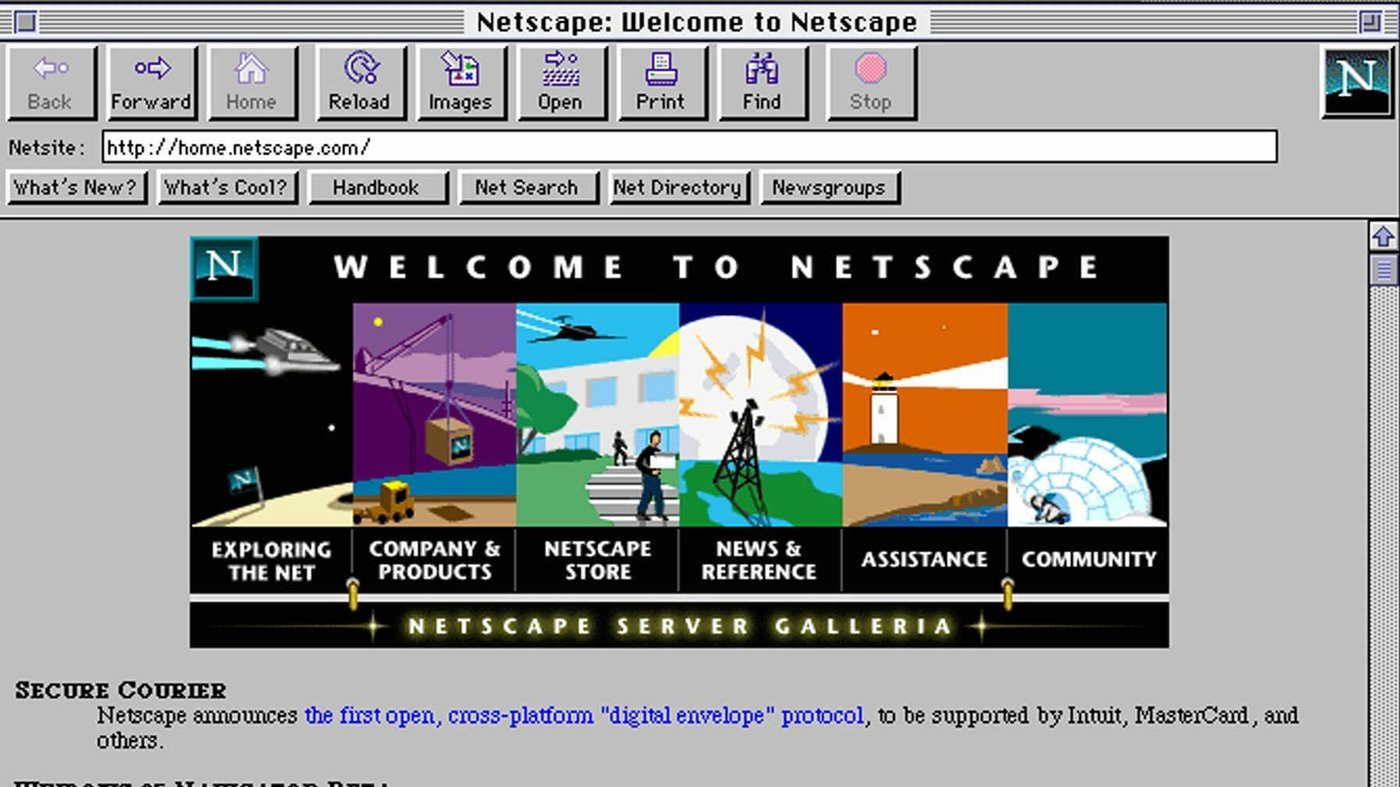
\includegraphics[width=\textwidth]{figures/002.jpg}
    \caption{Screenshot of the Netscape start-page \citep{npr_home_nodate}}
    \label{fig:netscape}
  \end{figure}

  That was the reason they hired the experienced programming language and network code developer Brendan Eich. Brendan’s first task was the nearly unachievable goal of creating such a scripting language for the web — due in 10 days. They (later) called it: JavaScript \citep{severance_javascript_2012}.

  \section{JavaScript’s Destiny}
  \label{sec:javascript-destiny}

  I don’t need to dig too deep into the history of the web to show you one crucial pain point of today’s web technology standards: JavaScript is a scripting language for the browser to interpret. I repeat it: JavaScript is a scripting language for the browser to interpret — not some fancy multi-paradigm system programming language that focuses on speed, security or code maintainability. It was supposed and designed to be an easy-to-understand dynamically-typed scripting language to give your website some cool DOM manipulations and decorative animations.

  Nevertheless, see what happened:

  \begin{quote}
    \emph{Any application that can be written in JavaScript, will eventually be written in JavaScript. – Jeff Atwood}
  \end{quote}

  A quote by Jeff Atwood (co-founder of Stack Exchange) that is popularly referred to as Atwood’s Law \citep{atwood_principle_2007}. Ever since frameworks like NodeJS or React Native became widely used, JavaScript’s possibilities already crossed the border of just living on the client-side inside of a browser. It’s nearly everywhere.

  Also, NodeJS’ NPM package manager is currently the most prominent and most active package registry platform ever created. As an example: From May 10th to May 17th of 2018, JavaScript developers downloaded 5.2 billion NodeJS packages from the NPM registry, setting a new record \citep{npm_inc_how_2018}

  \begin{figure}[ht]
    \centering
    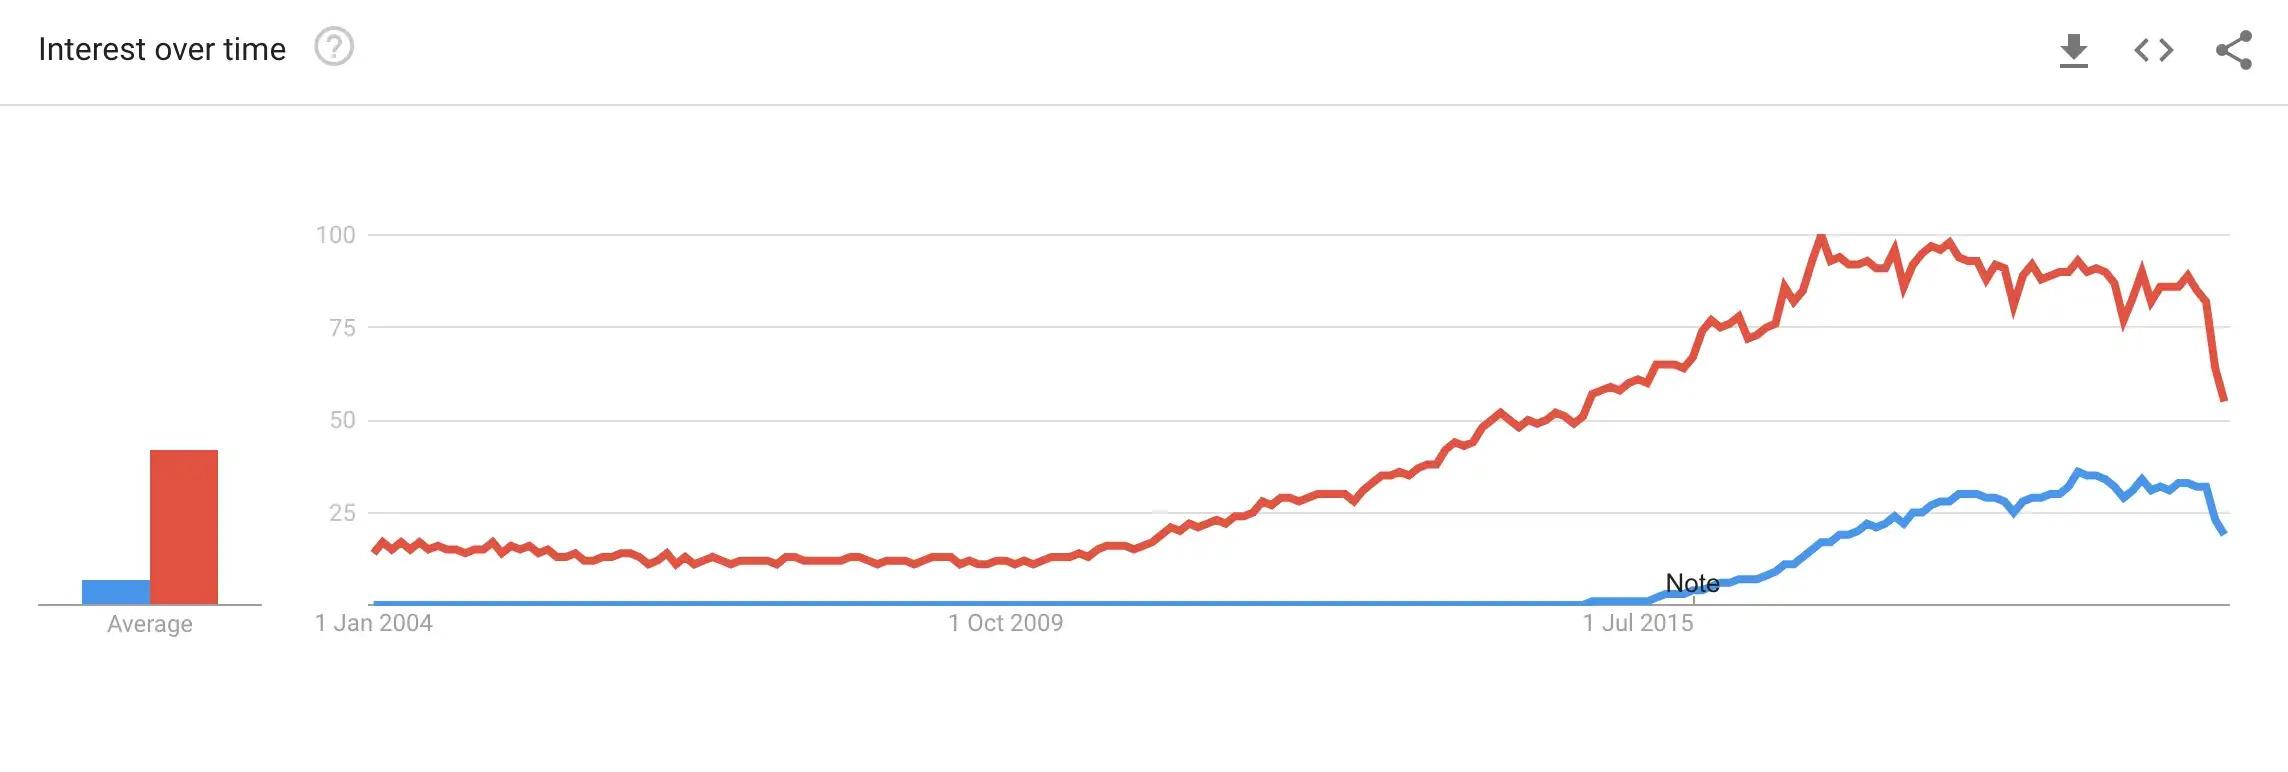
\includegraphics[width=\textwidth]{figures/003.jpg}
    \caption{Google Trends curve about NodeJS and React Native}
    \label{fig:atwood-law}
  \end{figure}

  \section{Treacherous Atwood’s Law}
  \label{sec:atwood-law}

  There are thousands of courses, books and tutorials on how to learn JavaScript. Every computer-related school now or then teaches JavaScript. Nearly everyone could be able to learn it anywhere with a minimum amount of effort. If you search for “Learn JavaScript” on Google, you’ll get \num{2220000000} search results. In comparison: When you search “Learn Java” you’ll get \num{305000000} results.

  Though, is that a good thing? Is an originally lightweight scripting language capable of ruling the world of computational web development? My opinion: No, it’s not, and I believe there won’t be such a bright future for JavaScript as nearly everybody claims. Let me explain it with a Harry Potter analogy:

  \section{Muggles Entering Hogwarts}
  \label{sec:muggles}

  Do you know how it feels to watch front-end developers call themselves “full-stack software developer” after they’ve simply learned NodeJS? It feels like Muggles entering Hogwarts—a school full of wizards. Only that in our case these wizards are trained software engineers and computer scientists. These are the people who learn all the hardcore-implemented algorithms and compilers, programming languages and operating systems. They know precisely how to build software \citep{might_what_2011}.

  \begin{quote}
    \emph{Do front-end developers know how to write actual software? I’d say we better don’t talk about it.}
  \end{quote}

  Muggles aren’t invited to Hogwarts because they have no magical ability. Front-end developers weren’t “invited” for software engineering too because they couldn’t even do something with the languages they knew. Nevertheless, now — thanks to all the cross-platform JavaScript runtimes — they’re suddenly here to do some magic. But imagine, what if the wizards of Hogwarts, our beloved software engineers and computer scientists, would be able to perform magic in the real world — or our case: the front-end? What would happen? What could go wrong?

  \section{WebAssembly Says Hello World}
  \label{sec:hello-world}

  \begin{figure}[ht]
    \centering
    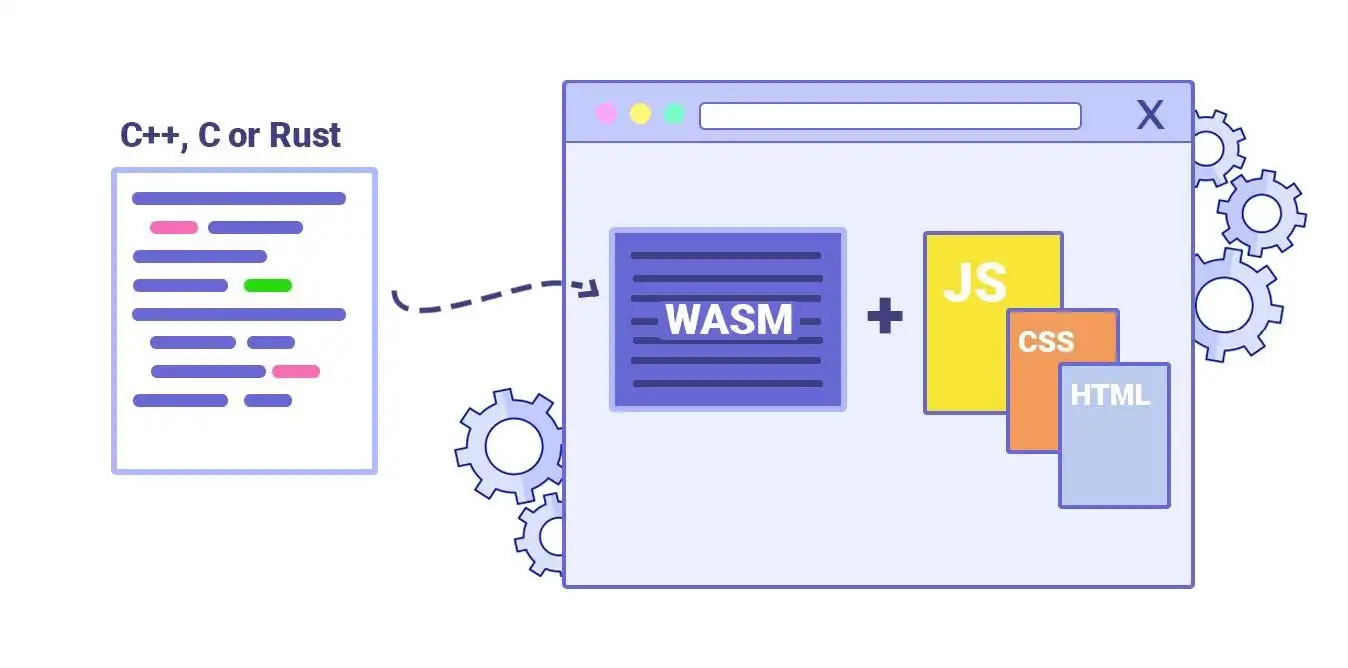
\includegraphics[width=\textwidth]{figures/004.jpg}
    \caption{Illustration of how WebAssembly modules are being delivered to the browser \citep{logrocket_logrocket_nodate}}
    \label{fig:wasm}
  \end{figure}

  WebAssembly is the new player in the web development industry. It’s fast, small, non-readable and not even a real programming language. Yes, you heard that right. You literally can’t code in WebAssembly \citep{rourke_learn_2018}. So I may hear you asking: Why should we all be excited about it? Well, as mentioned earlier, it’s a compilation byte-format target for high-level languages. You write your code in such a high-level language like C or C++ and compile it down to WebAssembly. The magic trick: It works in the browser, and it’s super fast — sometimes about 5 to 20 times faster than JavaScript \citep{aboukhalil_how_0200}.

  \section{WebAssembly in a Nutshell}
  \label{sec:in-a-nutshell}

  Enough with the marketing fuzz. The real face behind the term “WebAssembly” isn’t that uniform as it’s being marketed. WebAssembly itself is only a piece of a bigger technology chain of workflows and concepts. There are several other key components that are important for delivering super-fast web applications. It’s also good to know what its current limitations are and for which use cases it’s the best. But first, let me introduce you to the five key components:

  \subsection{WebAssembly in a Nutshell}
  \label{sec:webassembly-text-format}

  This is a human-readable file format you’ll get when you compile your C, C++ or Rust code. It represents the abstract syntax tree (AST) from the source code of a programming language. An AST — or in the WebAssembly case: a .wat file — may be verbose, but it does an excellent job at describing the components of source code. Representing source code in an AST makes verification and compilation simple and efficient. Here is a simple return function called \lstinline{getDoubleNumber} written in C:

  \begin{lstlisting}[language=C, caption=Python example, label=lst:python-example]
int getDoubleNumber(int number) {
  return number * 2;
}
\end{lstlisting}

  \pagebreak
  \bibliographystyle{references/custom-apa}
  \bibliography{references/bibliography}
\end{sloppypar}
\end{document}